\subsection{Temperatures on a day}
The member function \texttt{tempOnDay()} (corresponding to the \texttt{class tempTrender}) creates a histogram with the temperatures recorded for a specific day given as an input by the user. It tries to fit the histogram with a Gaussian distribution as well. An example for this is shown in Figure \ref{fig:LundTeml}. In the figures, one can see the change in mean temperature and spread through the different months. This indicates how the temperature distribution changes with the seasons. During summer, around June-September the temperature is much higher compared to winter, around December-March. 
\begin{figure}[H]
    \centering
    \subfloat[March 6th]{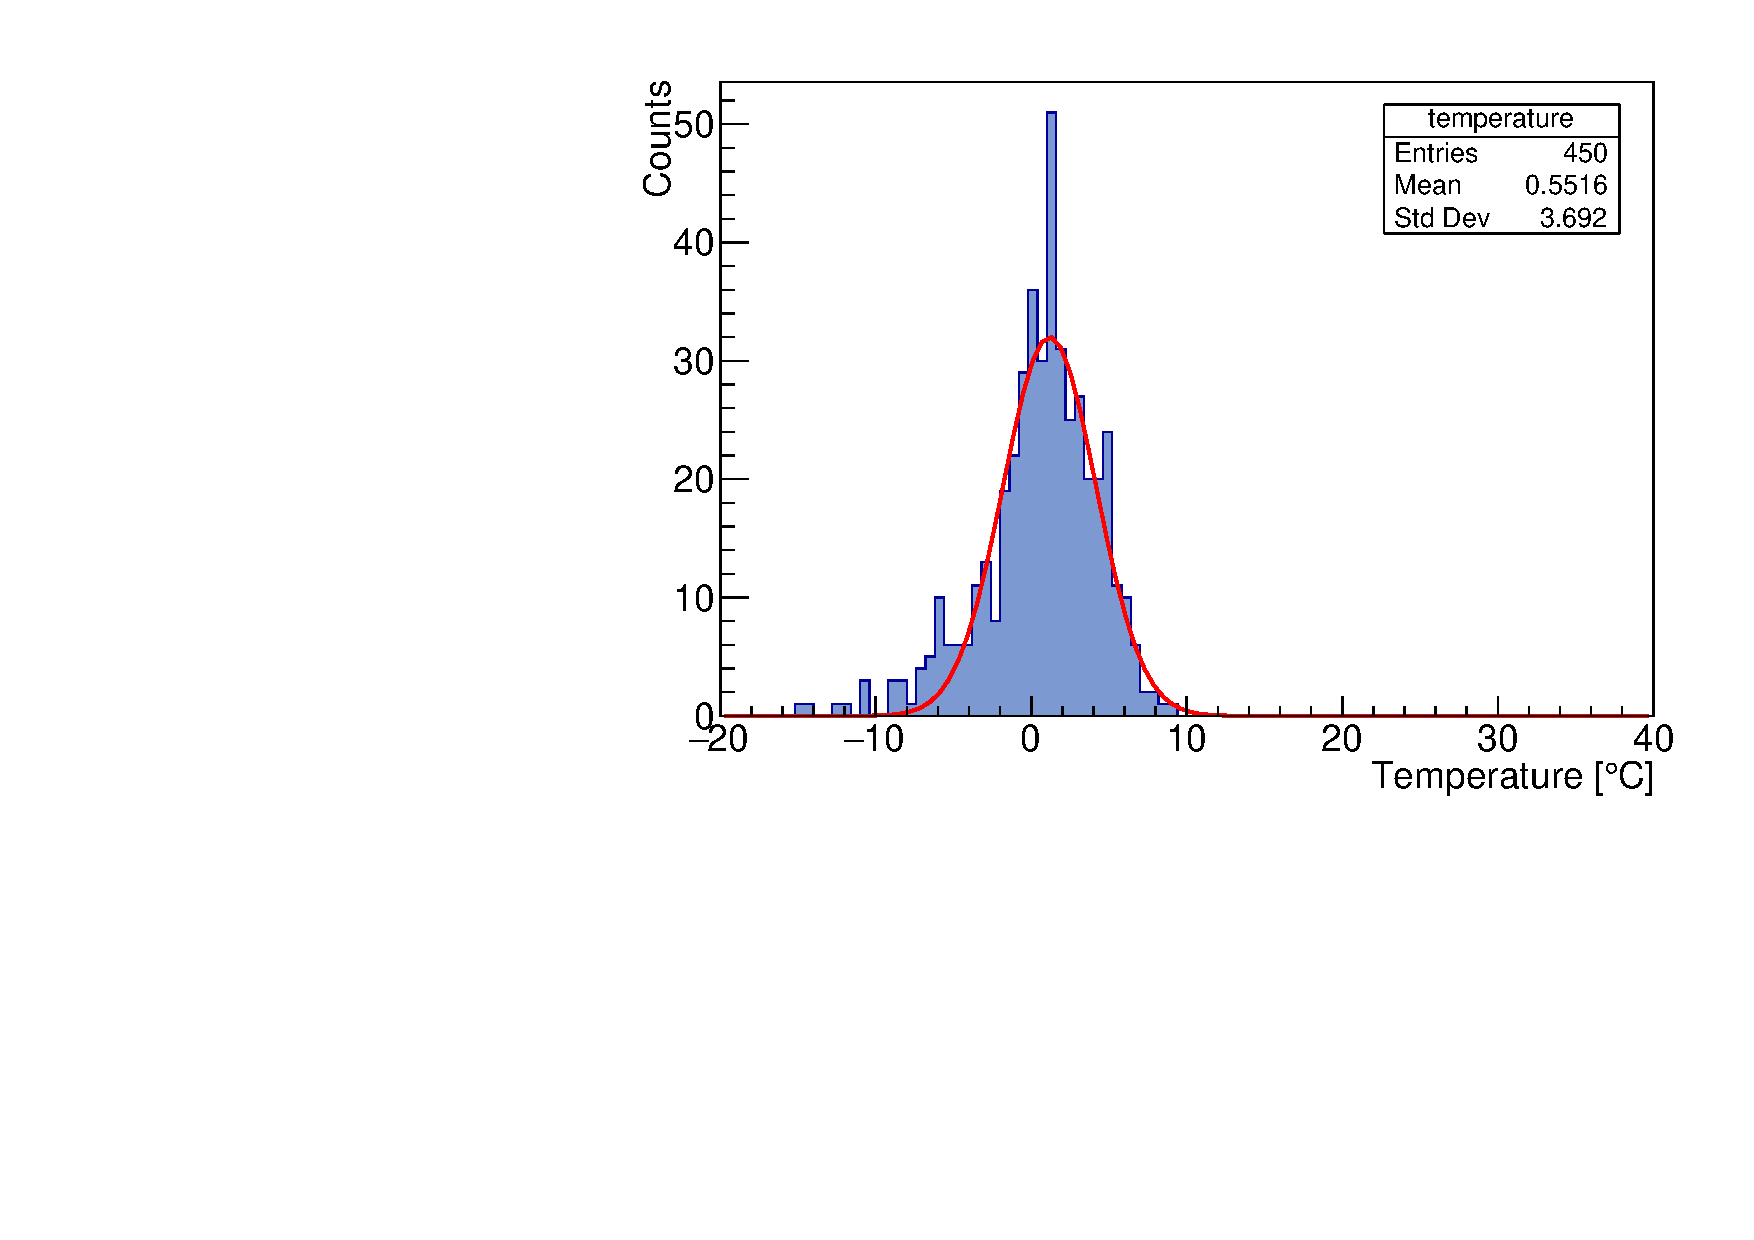
\includegraphics[width=0.49\linewidth]{Images/Lund3-3.pdf}}
    \subfloat[June 6th]{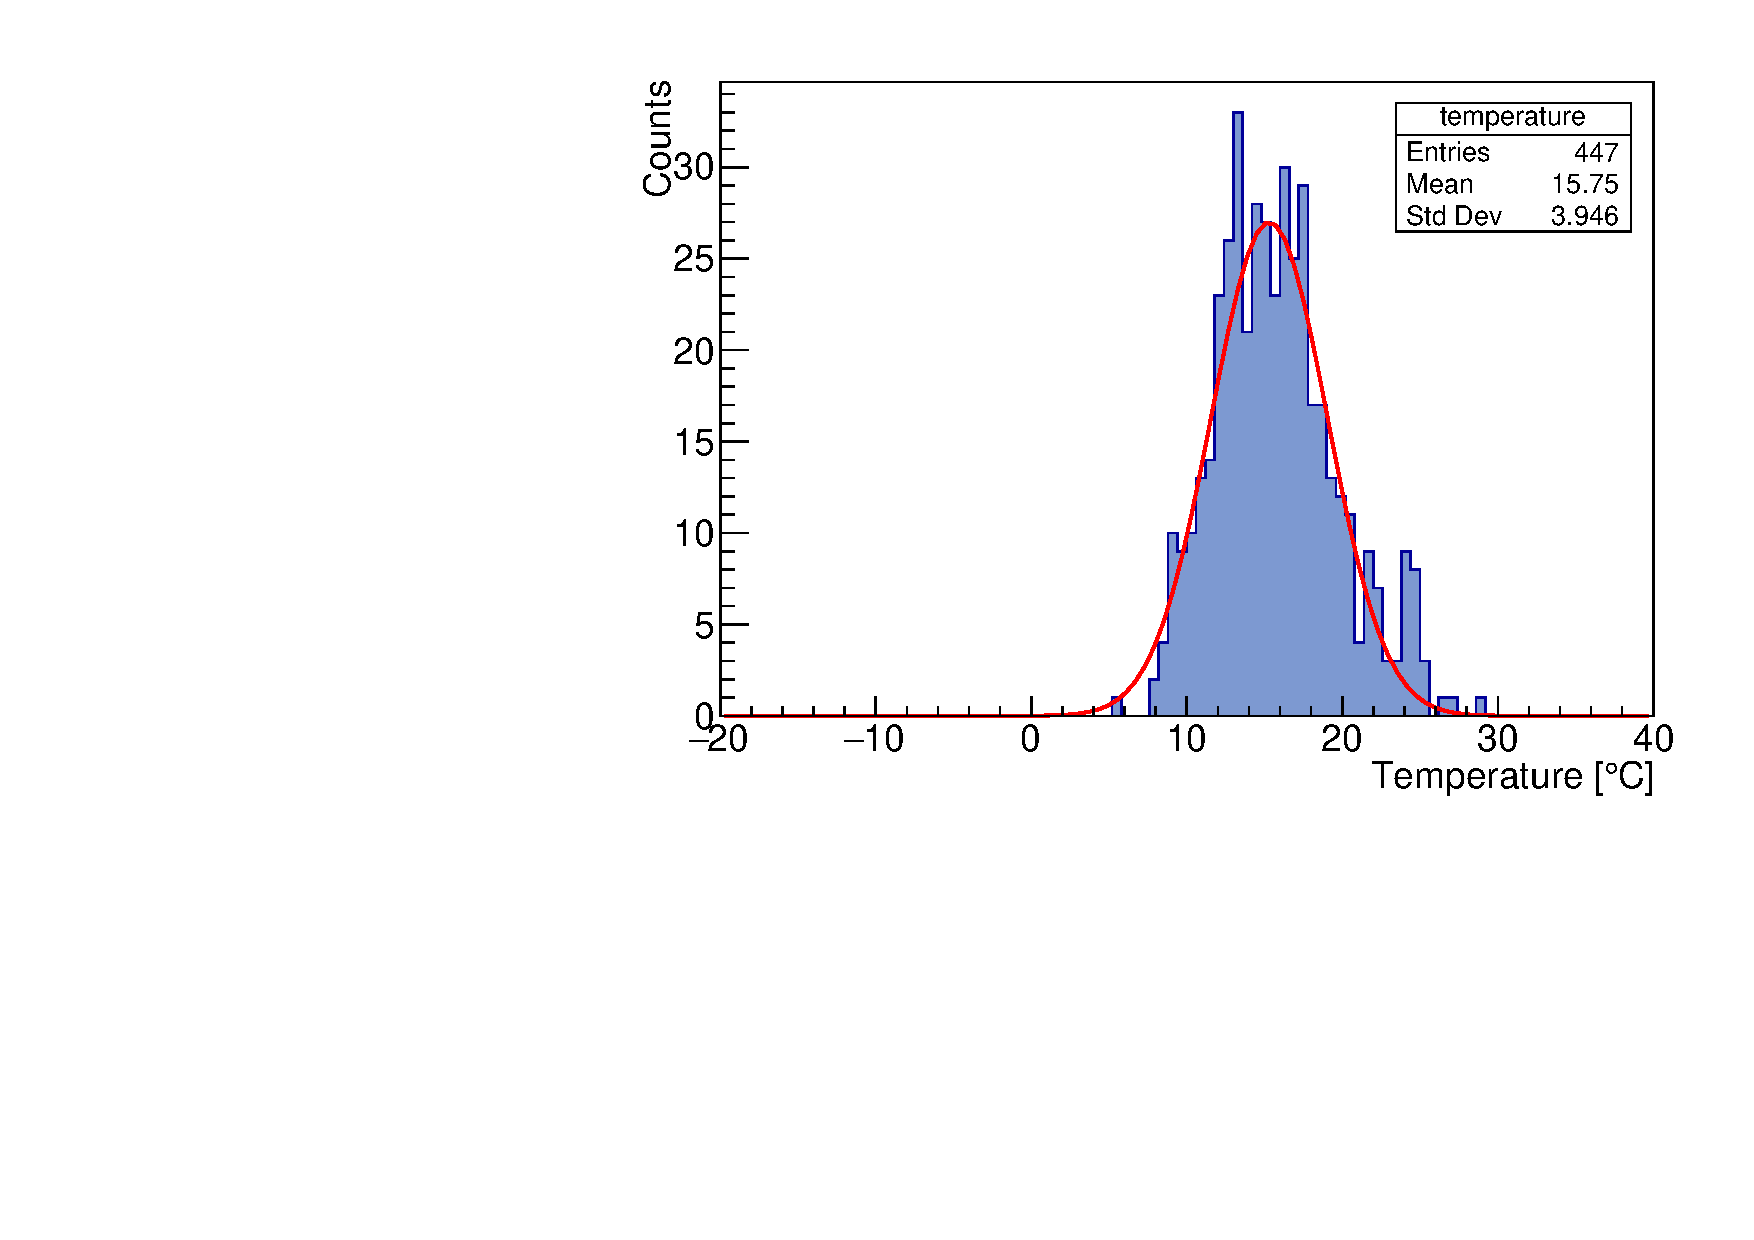
\includegraphics[width=0.49\linewidth]{Images/Lund6-6.pdf}}
    \quad
    \subfloat[September 6th]{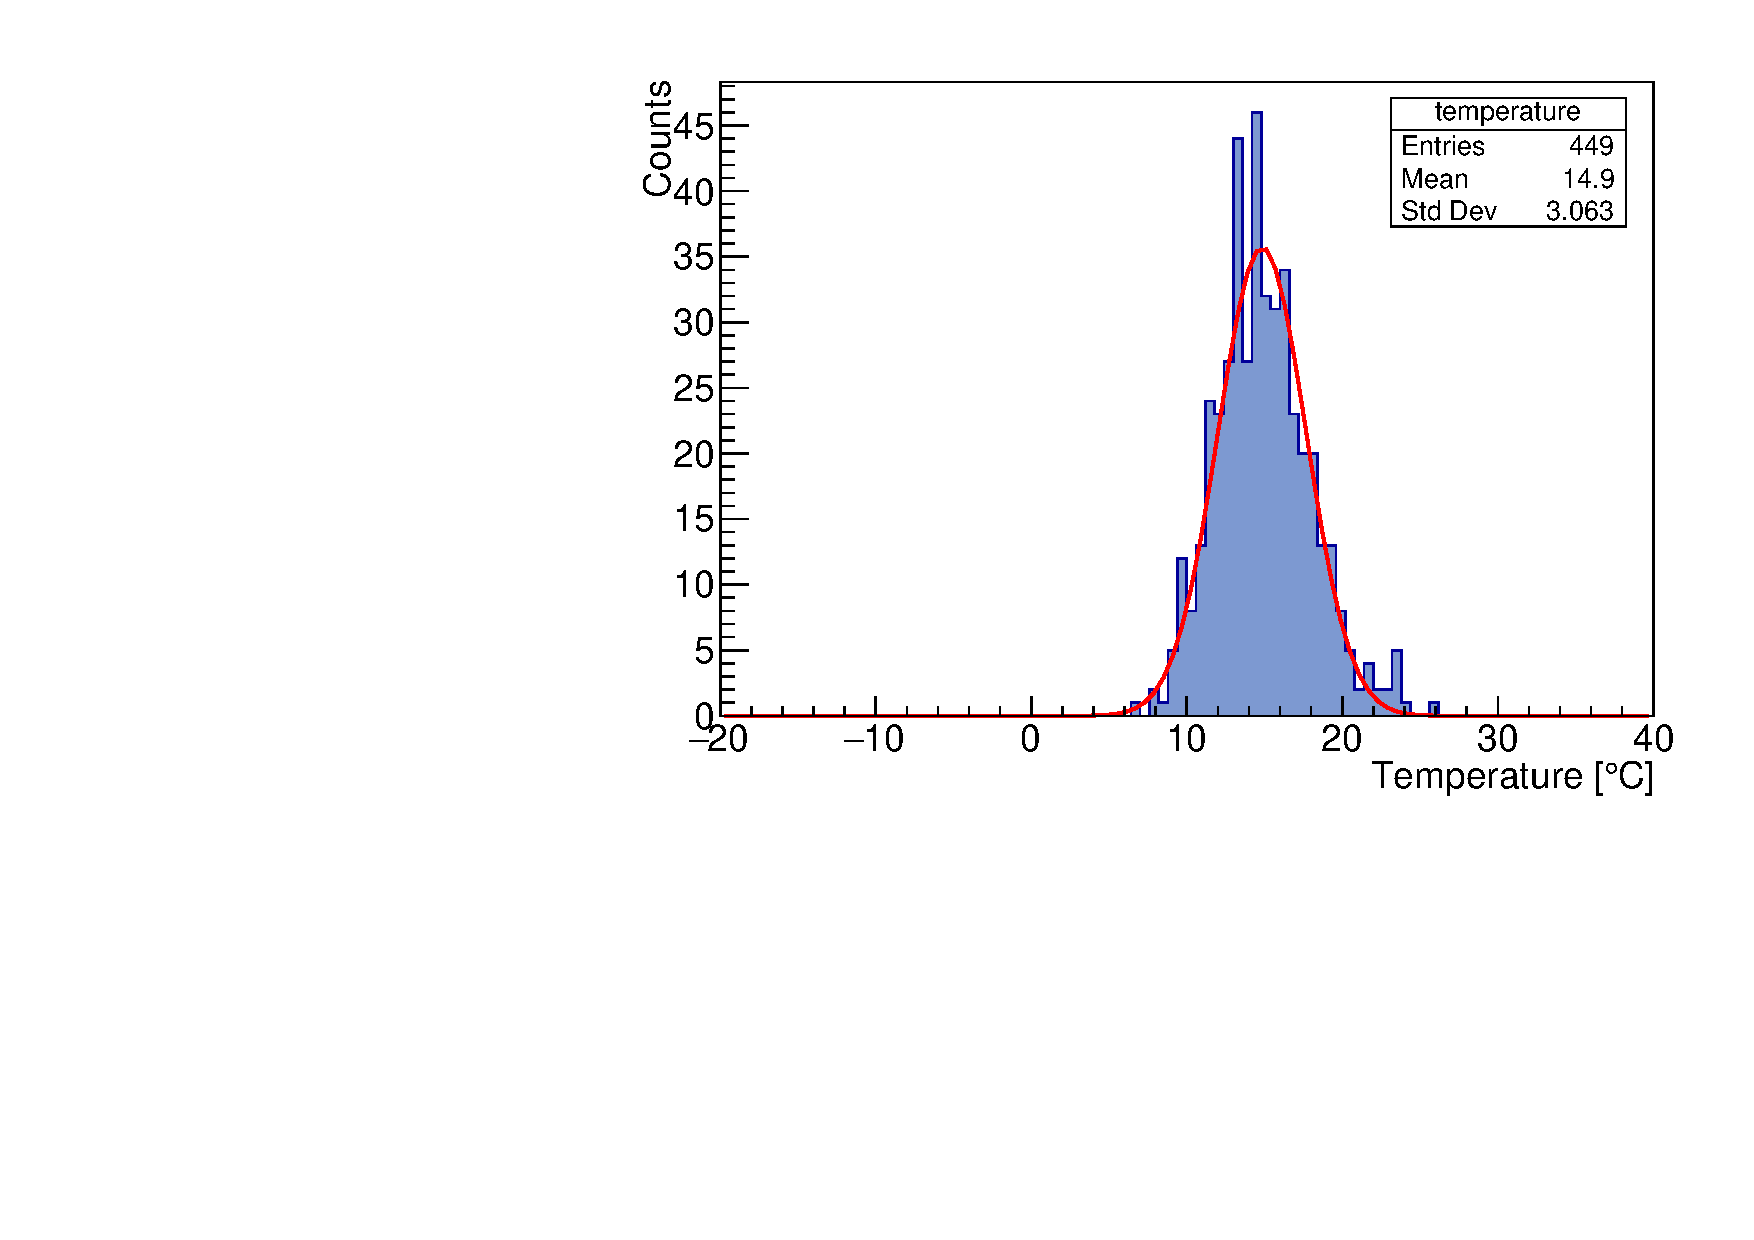
\includegraphics[width=0.49\linewidth]{Images/Lund9-6.pdf}}
    \subfloat[December 6th]{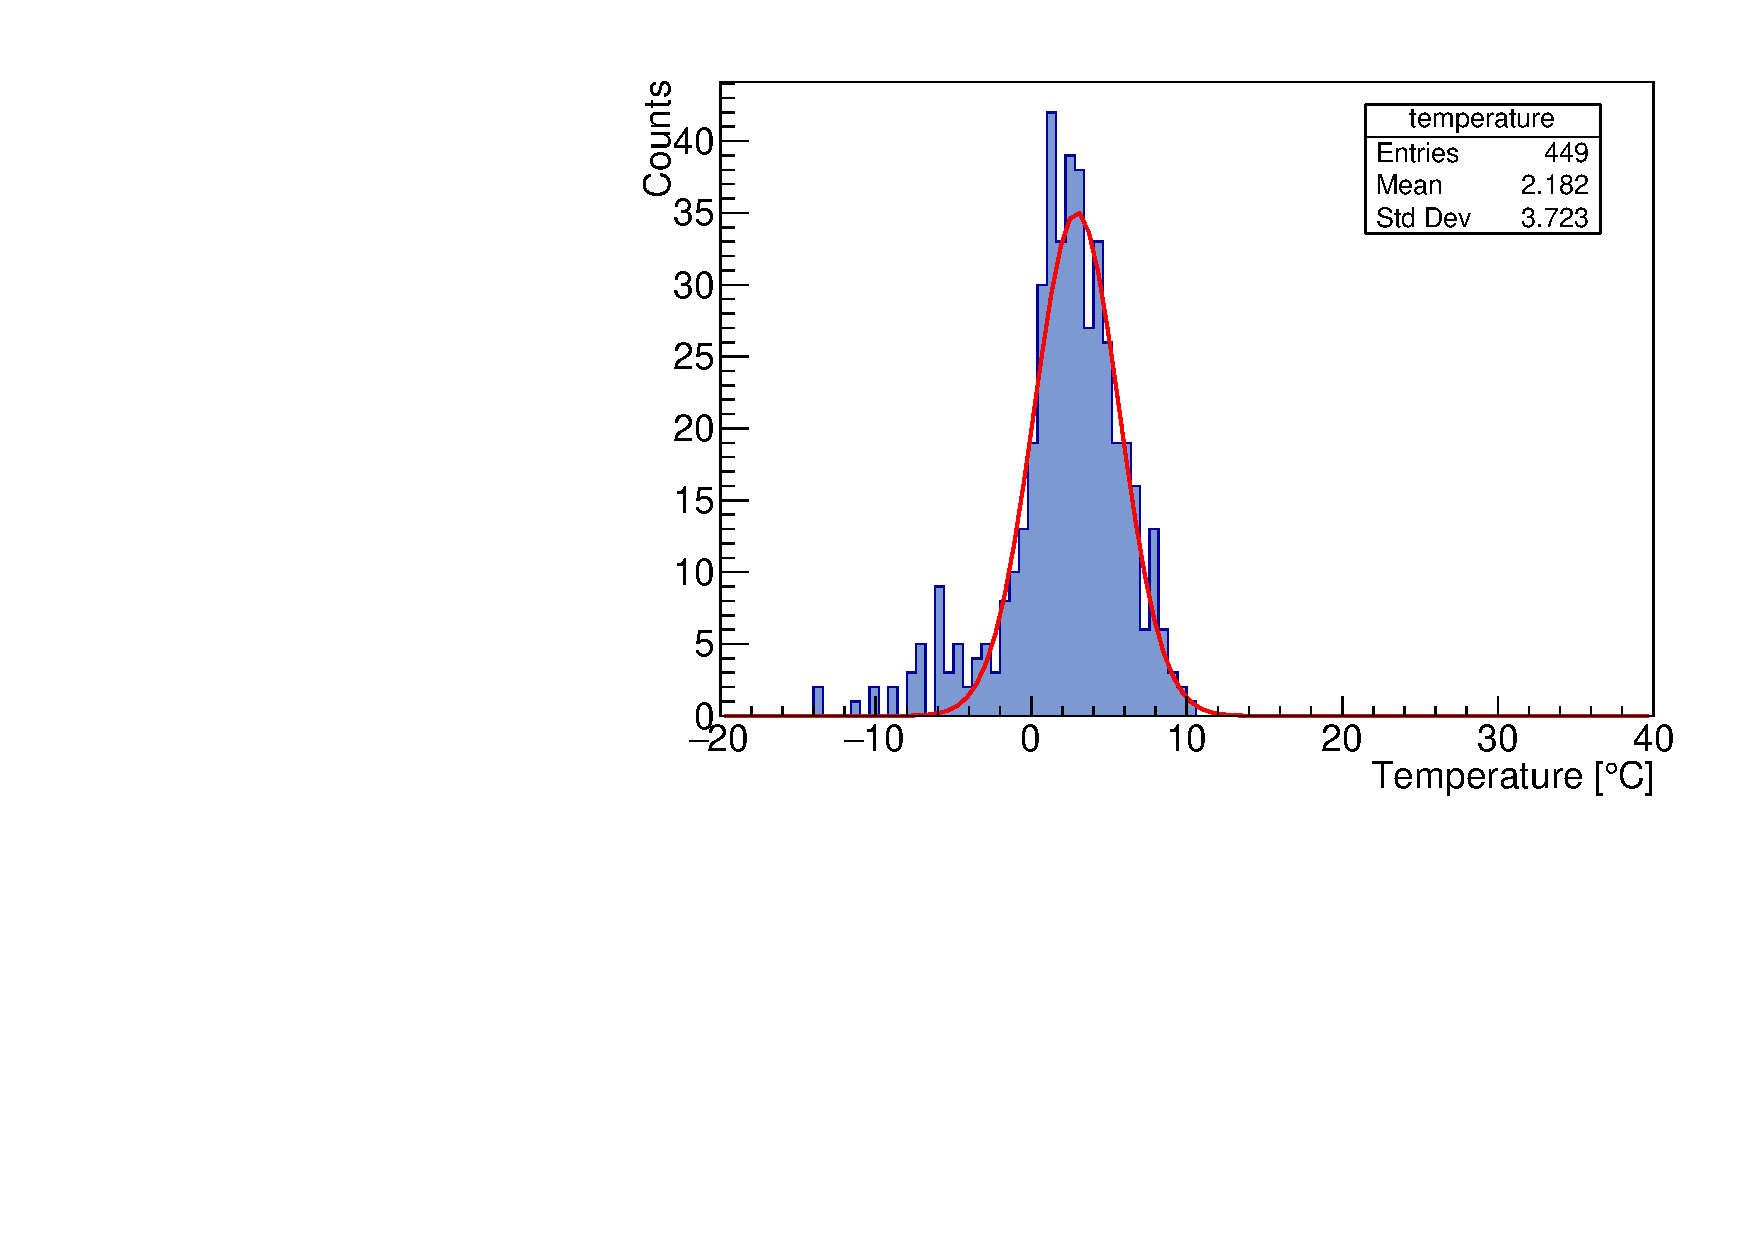
\includegraphics[width=0.49\linewidth]{Images/Lund12-6.pdf}}
    \caption{Temperatures in Lund}
    \label{fig:LundTeml}
\end{figure}

\noindent Since the distribution seemed normal, it was possible to use the ROOT fitting functions to do a gaussian fit and know the average temperatures as well as their standard deviations. The temperatures change over the year as expected and they have standard deviations from the average by 3-4 degrees. This is different to the case in cities which are located in the northernmost part of Sweden such as Luleå where the distribution is not quite normal. In Figure \ref{LuleåTemp}, we can see an almost exponential distribution and therefore the Gaussian fit does not provide any meanful information in this case. Although, the number of data points of temperatures measured might not have been enough to show the actual distribution which might be a Gaussian (as one can see the entries for Luleå were less than half than for Lund).



\begin{figure}[H]
    \centering
    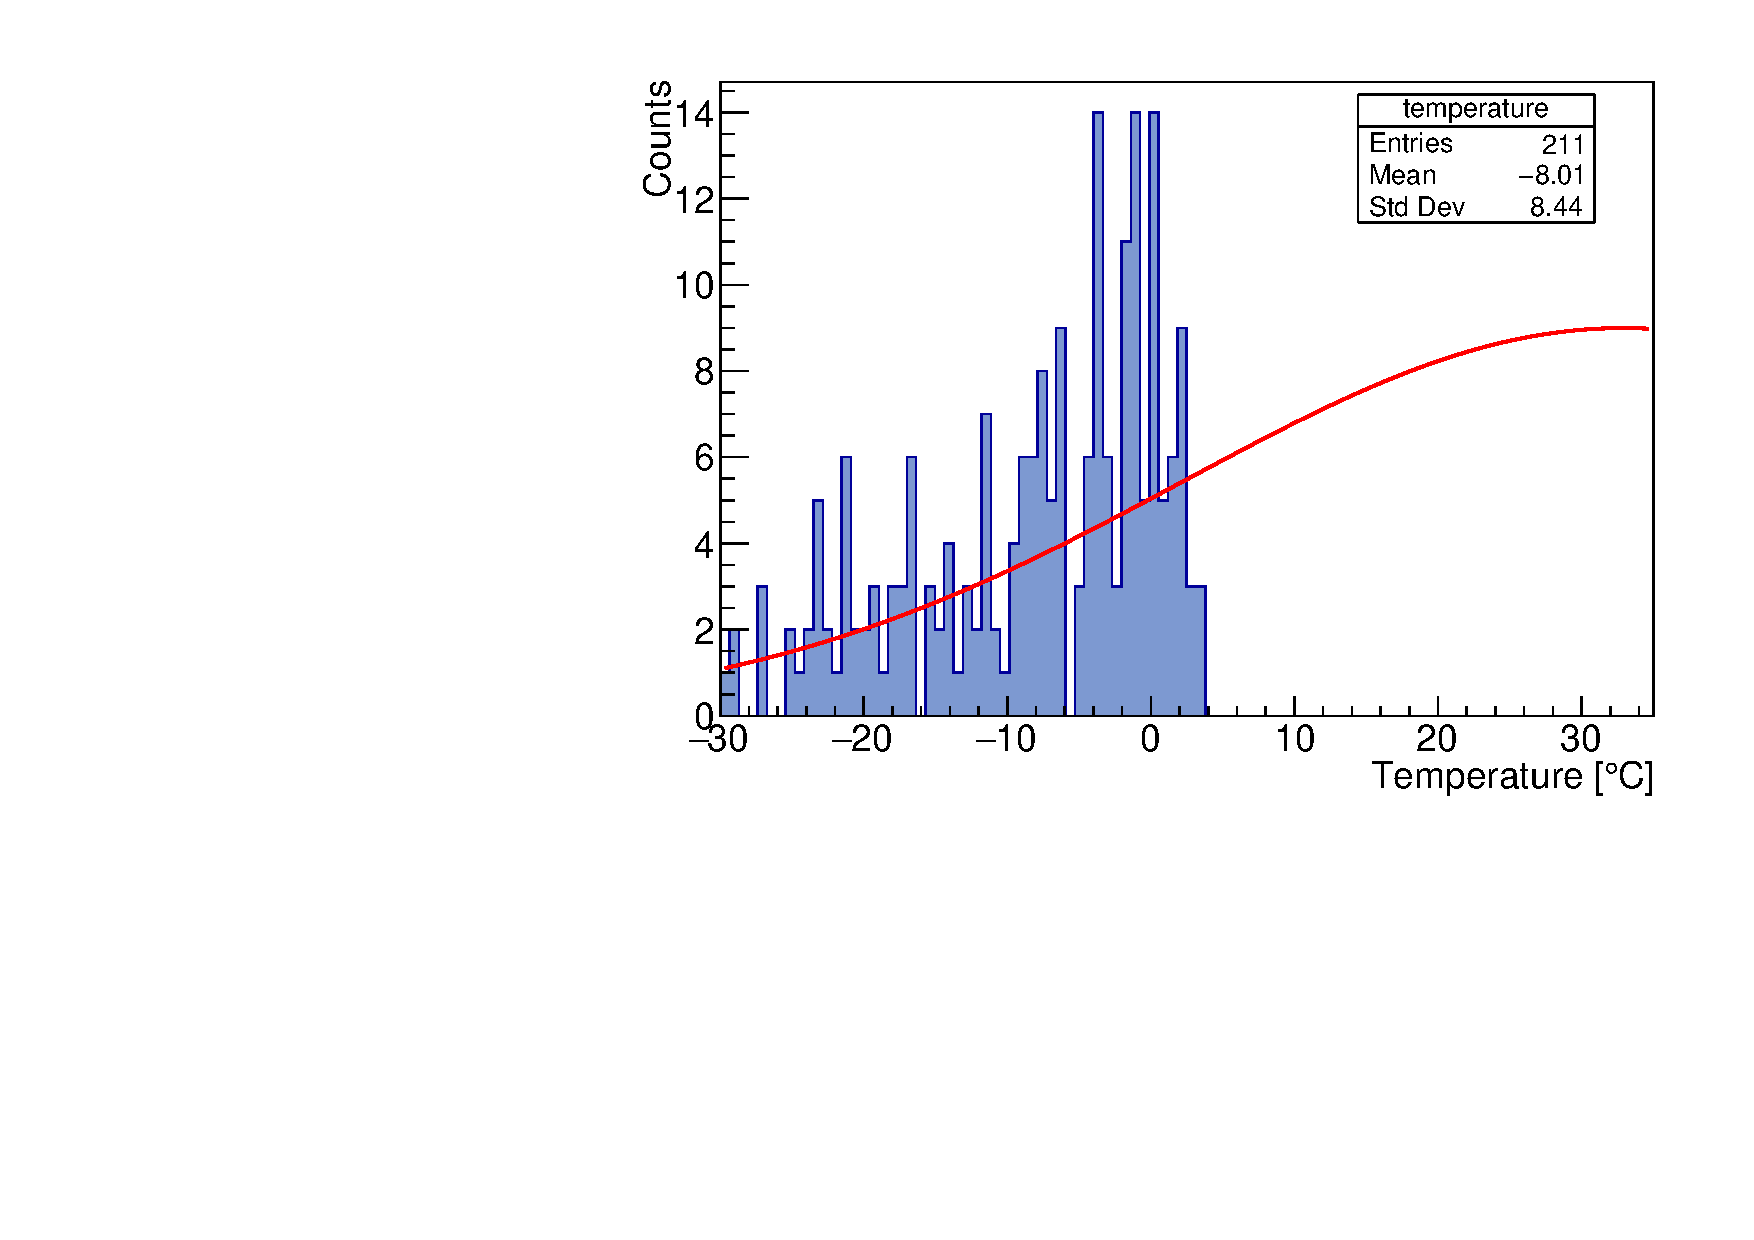
\includegraphics[scale=0.6]{Images/lulea_histogram.pdf}
    \caption{Histogram of the Temperature in Luleå on December 15}
    \label{LuleåTemp}
\end{figure}
One could also compare the temperatures for different cities for the same day as in Fig \ref{fig:Cities}. Although, the mean temperature is not that different for the different cities, it is noticed that as one goes more North the temperature drops slightly.

\begin{figure}[H]
    \centering
    \subfloat[Falsterbo]{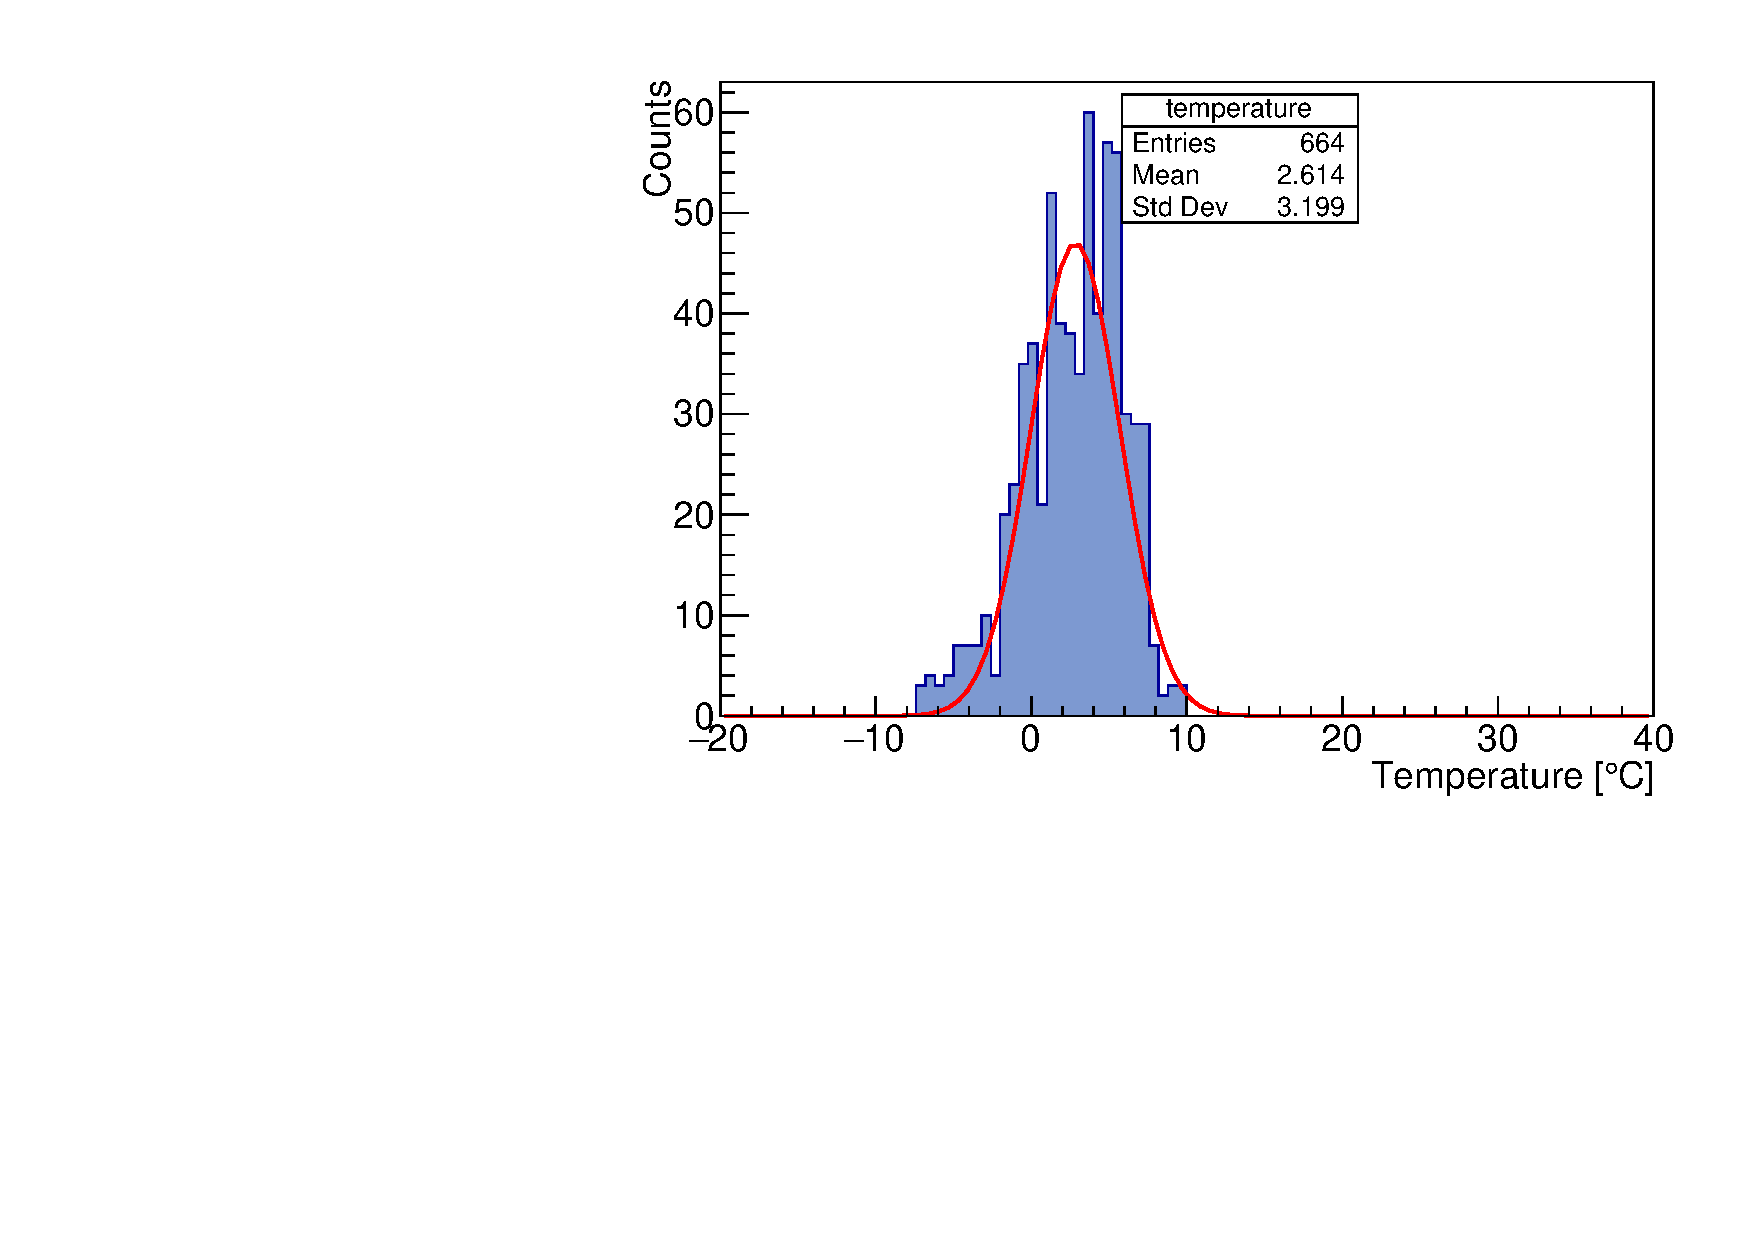
\includegraphics[width=0.49\linewidth]{Images/Task1Images/Falsterbo1215.pdf}}
    \subfloat[Borås]{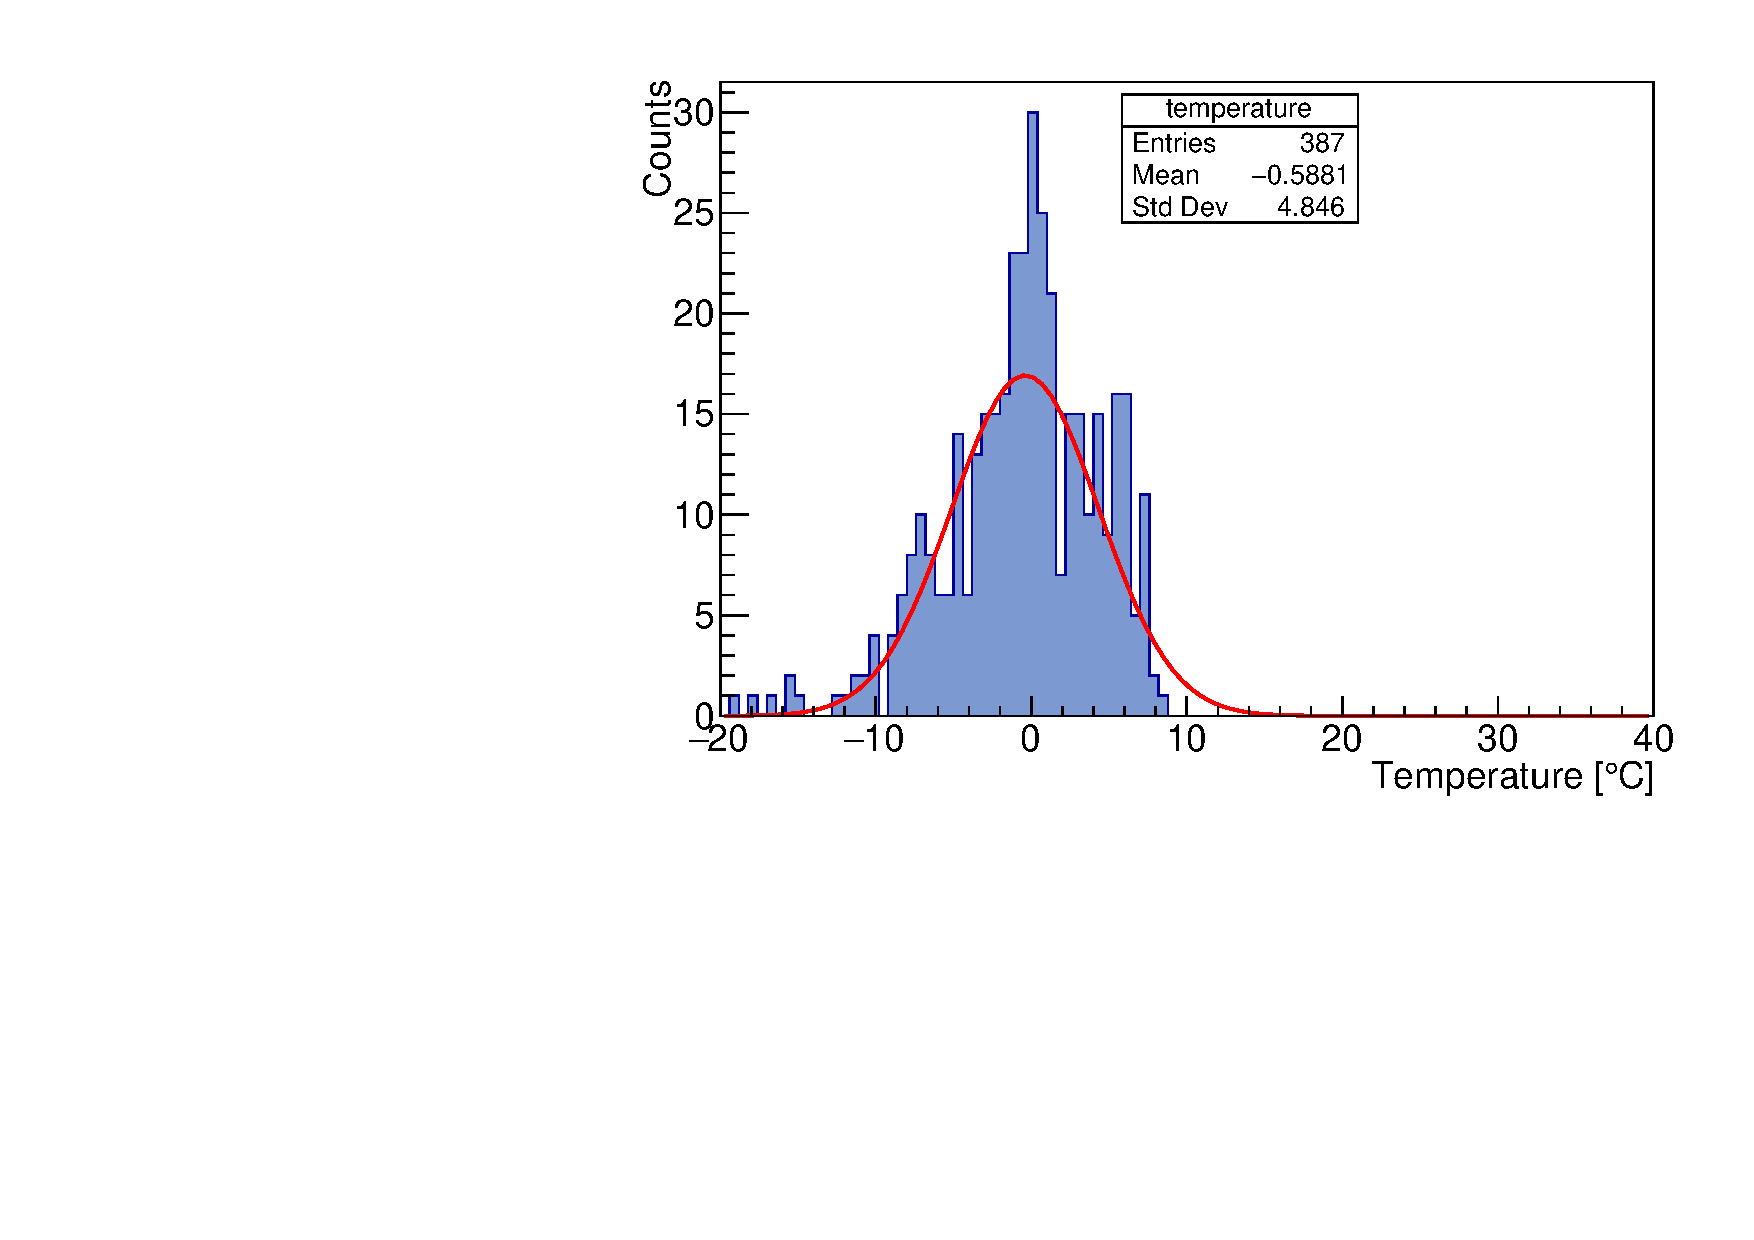
\includegraphics[width=0.49\linewidth]{Images/Task1Images/Boras.pdf}}
    \quad
    \subfloat[Karlstad]{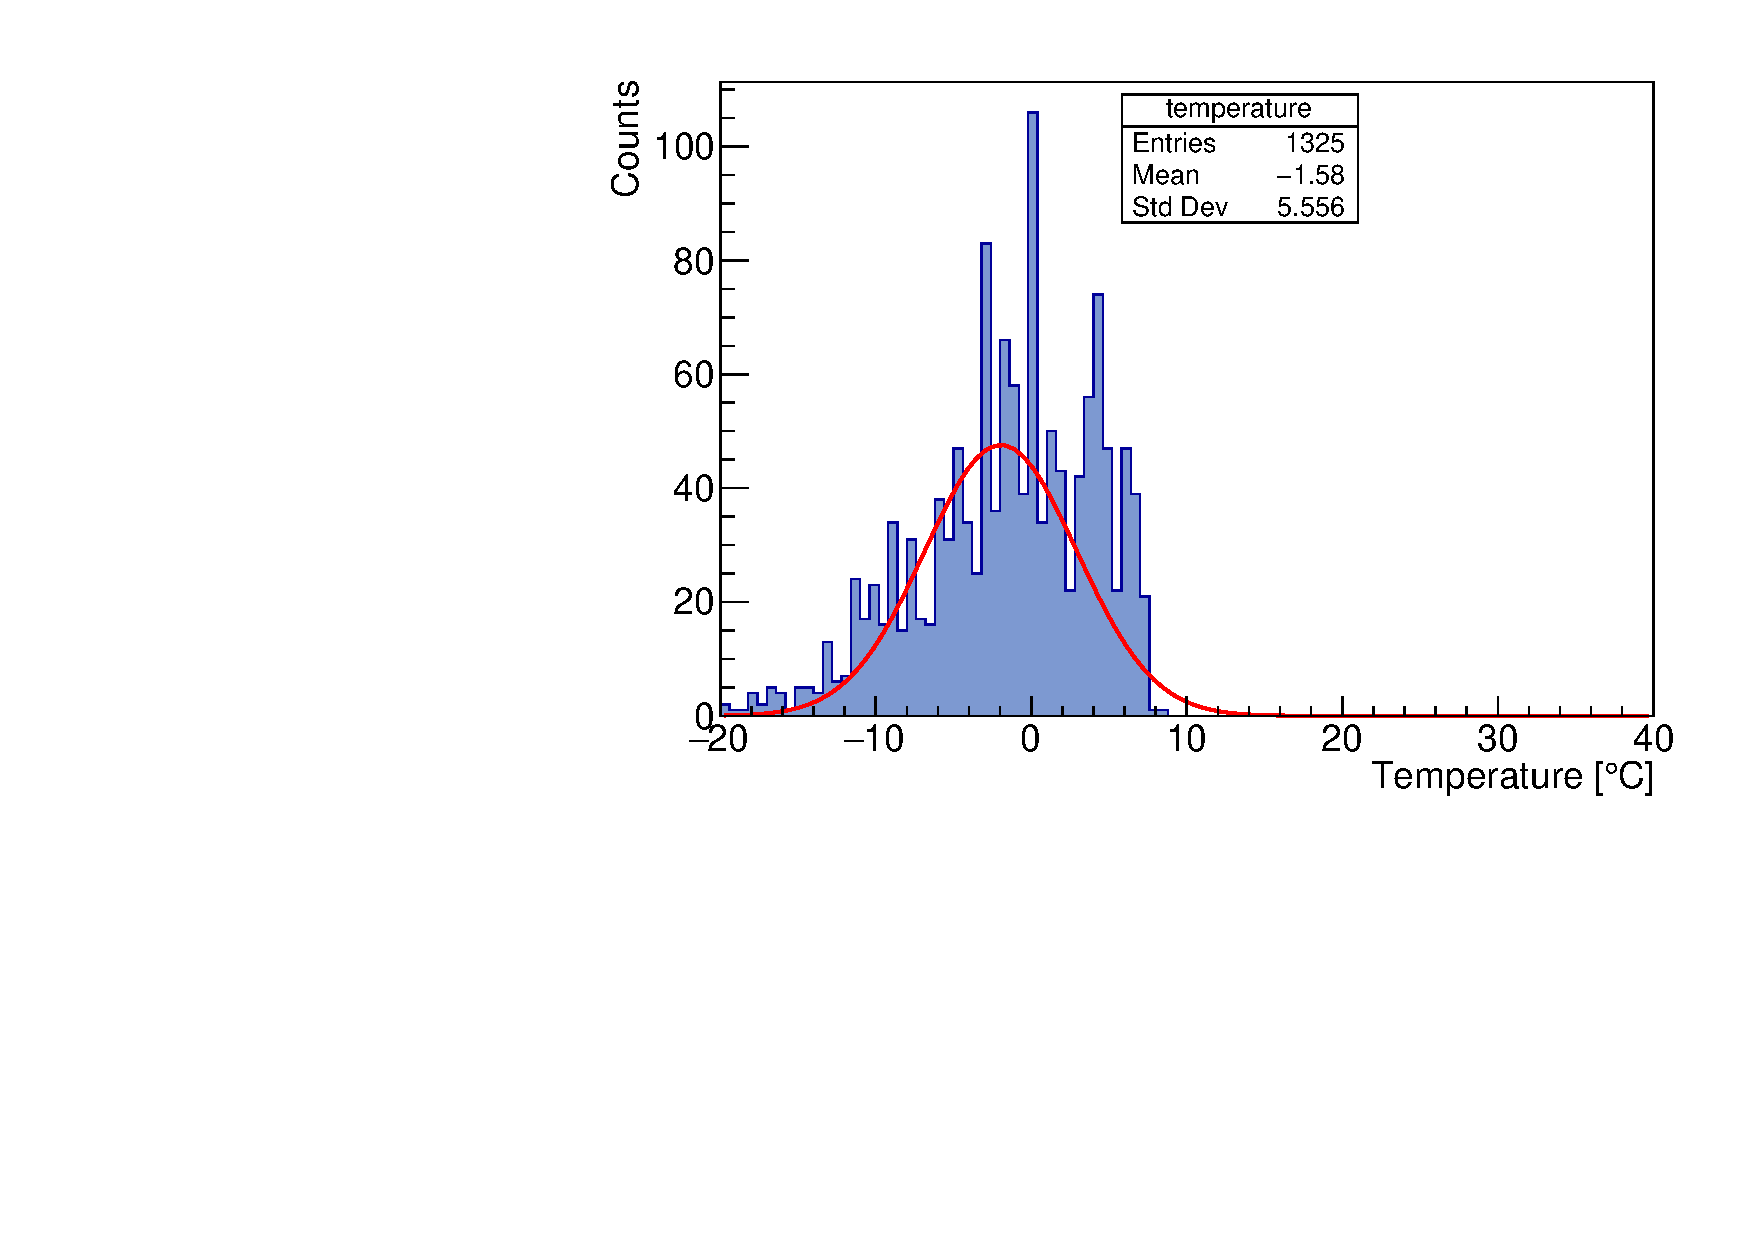
\includegraphics[width=0.49\linewidth]{Images/Task1Images/Karlstad1215.pdf}}
    \subfloat[Falun]{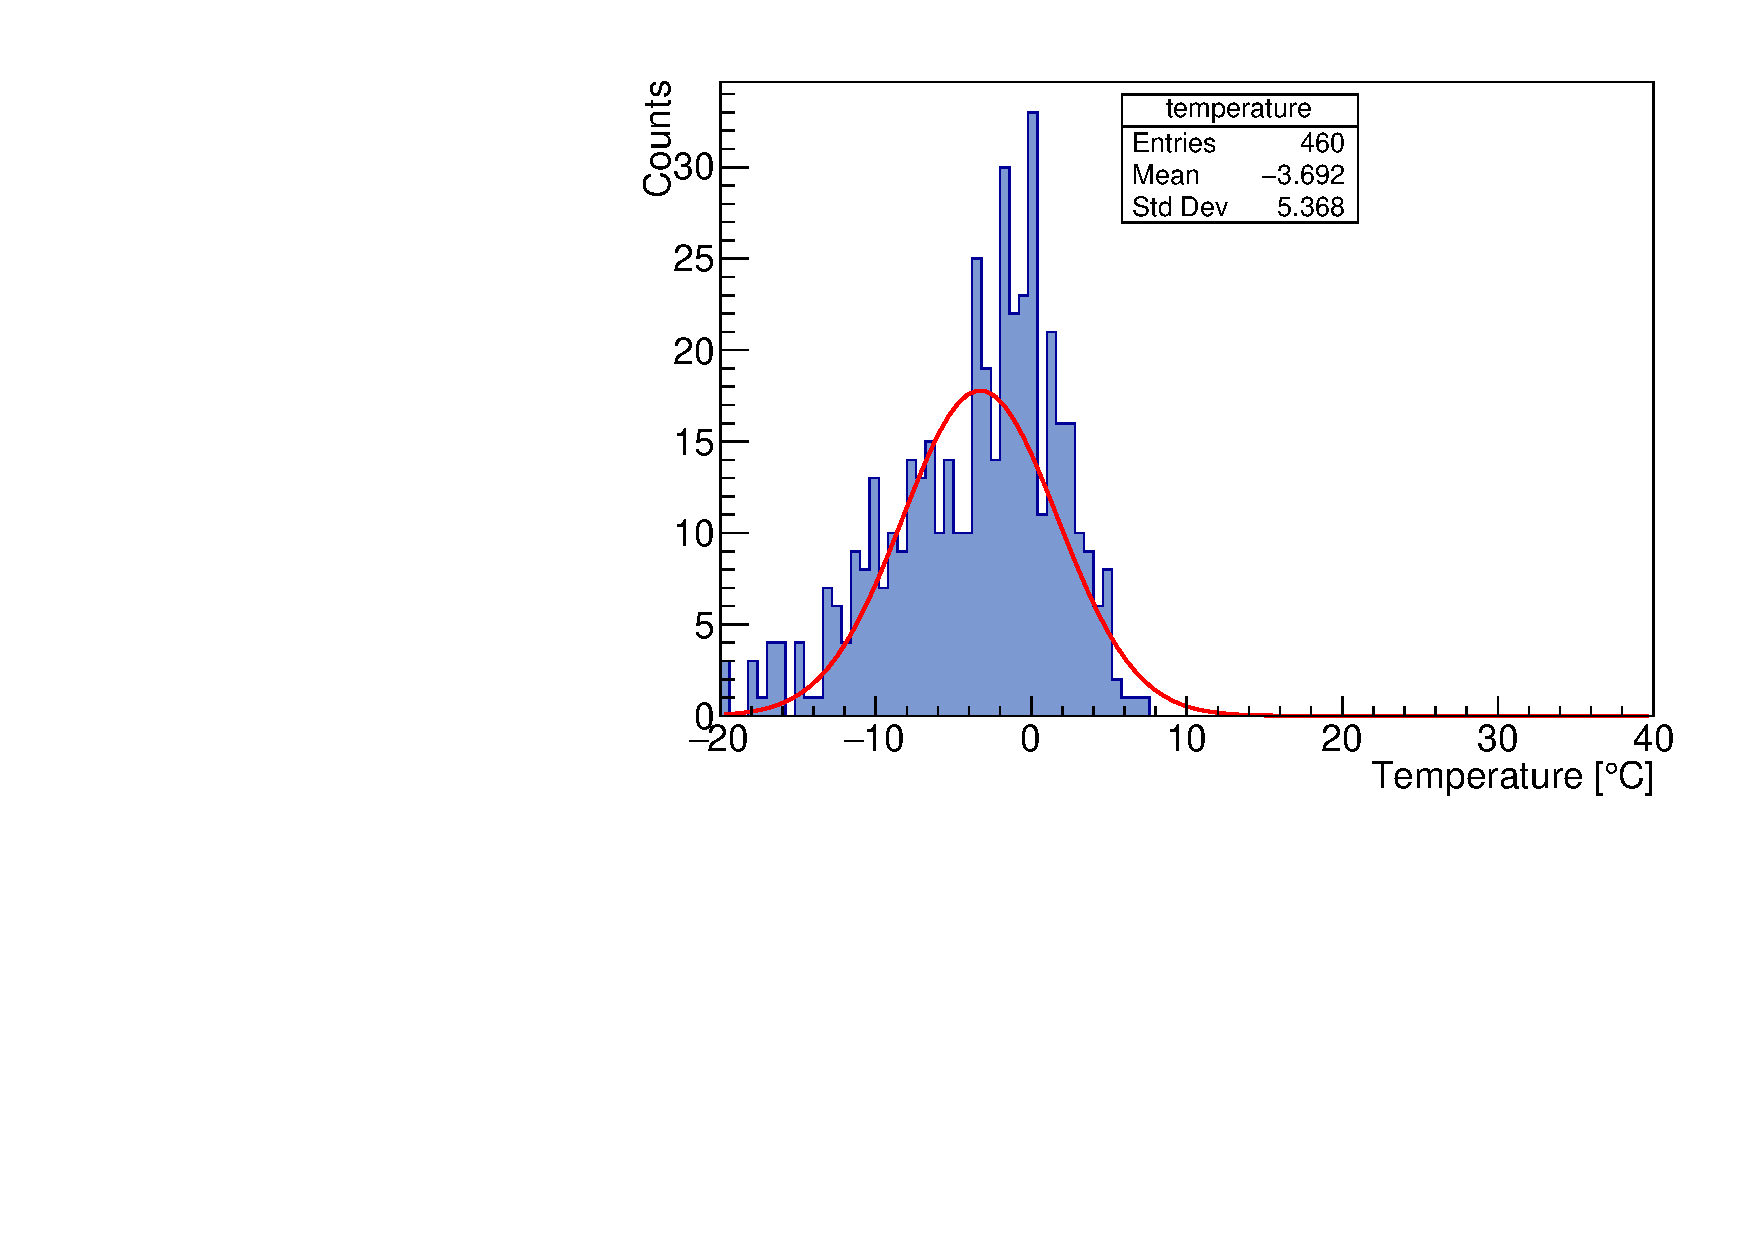
\includegraphics[width=0.49\linewidth]{Images/Task1Images/Falun1215.pdf}}
    \caption{Temperatures in different cities on December 15.}
    \label{fig:Cities}
\end{figure}

\newpage
\subsection{Yearly max and min temperatures}
In this part, the maximum and minimum temperatures for a given city were found and plotted over time. In figure \ref{fig:MinMaxTemp}, the maximum and minimum temperatures are given for 4 cities, Falsterbo, Lund, Borås and Umeå.
\begin{figure}[H]
    \centering
    \subfloat[Falsterbo]{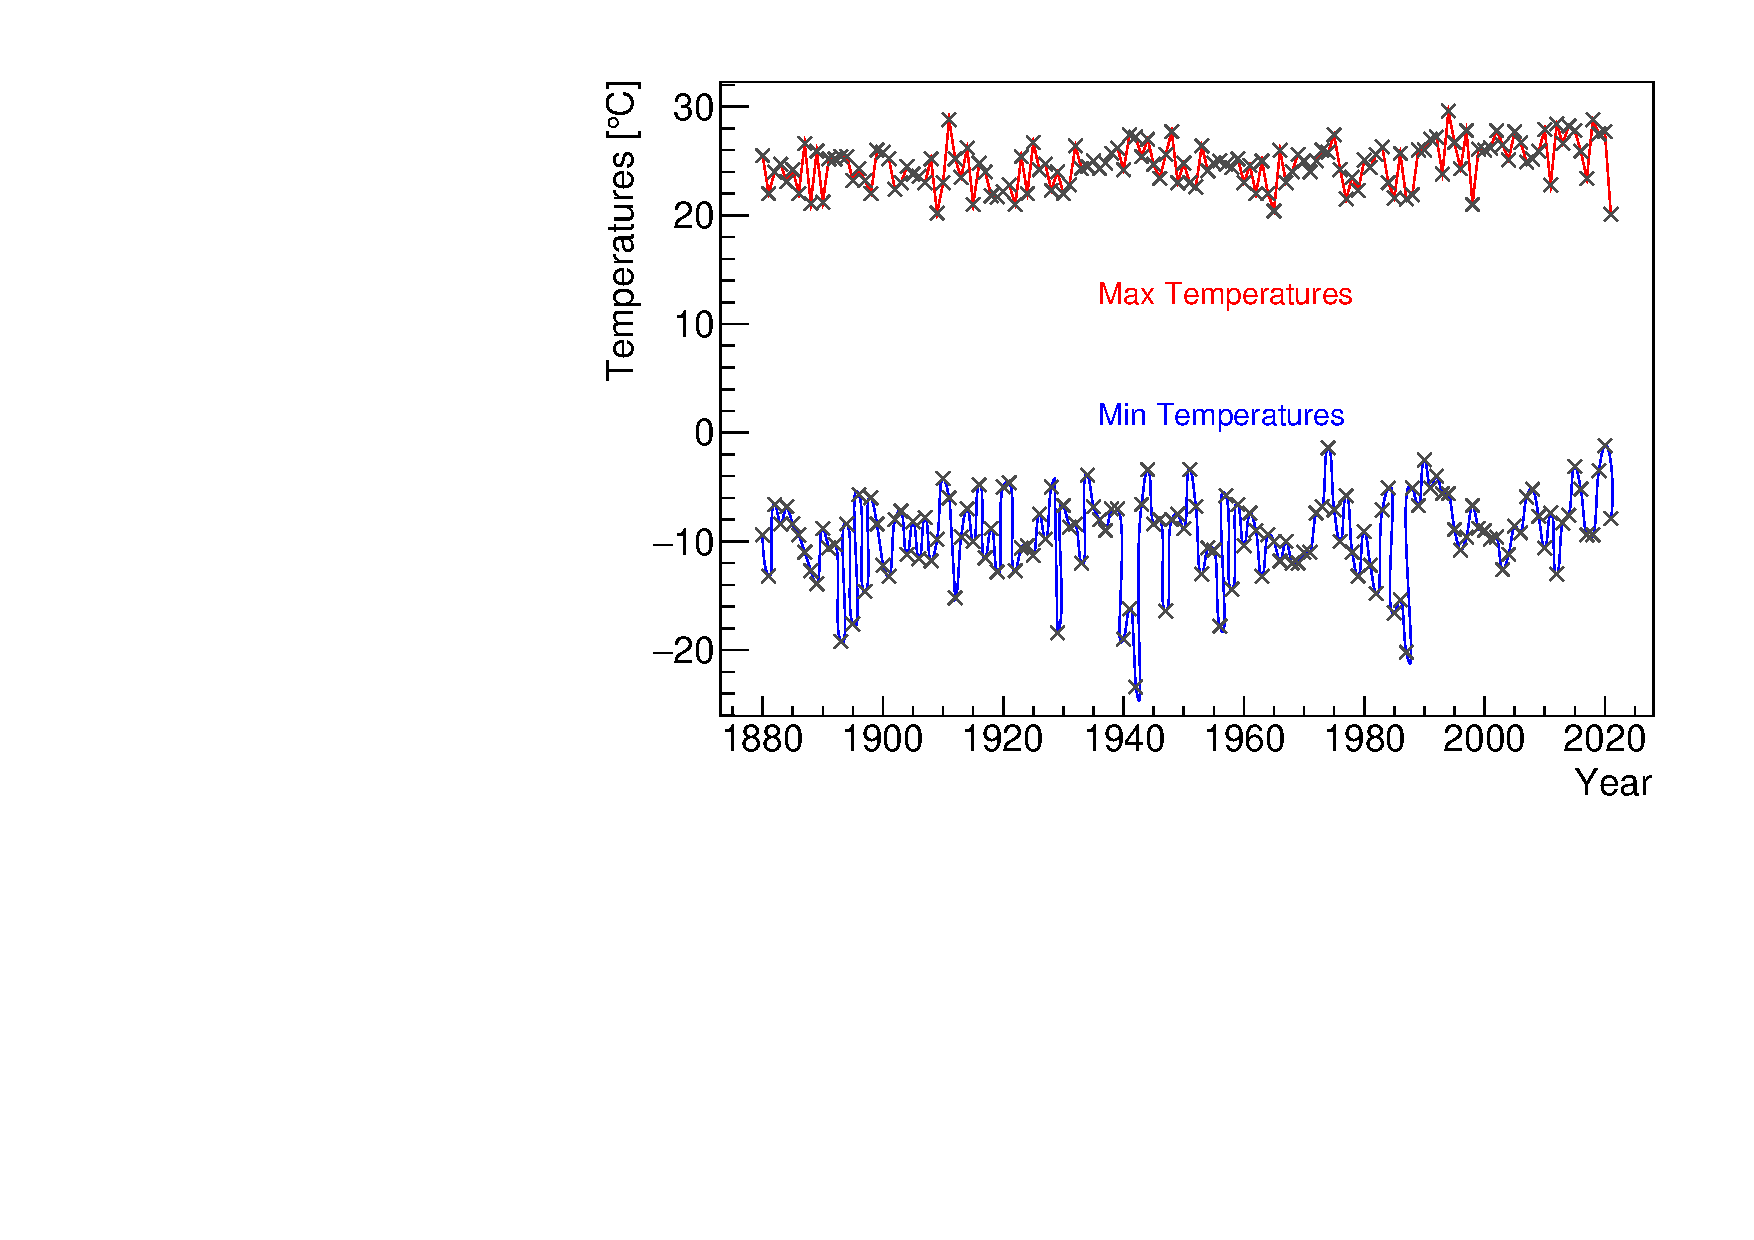
\includegraphics[width=0.5\linewidth]{Images/minmax_falsterbo.pdf}}
    \subfloat[Lund]{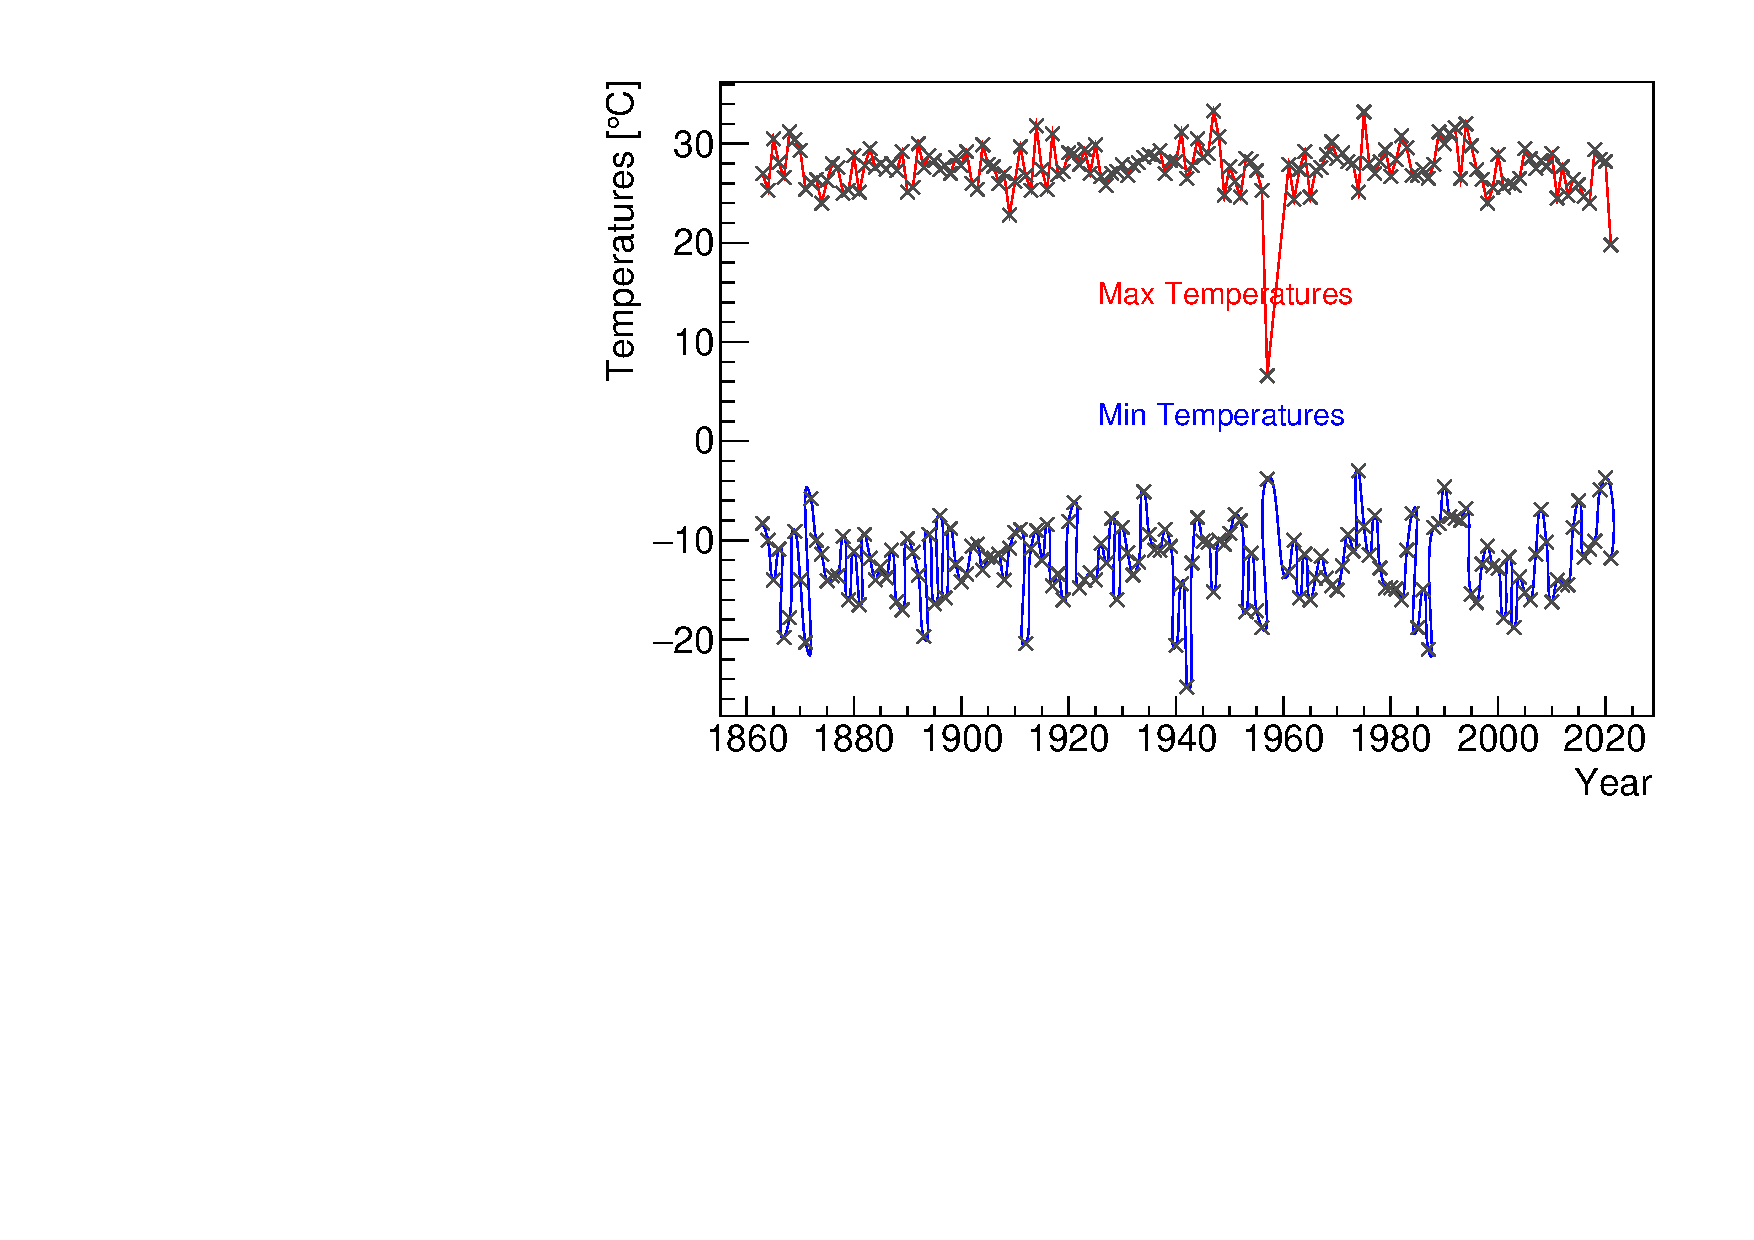
\includegraphics[width=0.5\linewidth]{Images/minmax_lund.pdf}}
    \quad
     \subfloat[Borås]{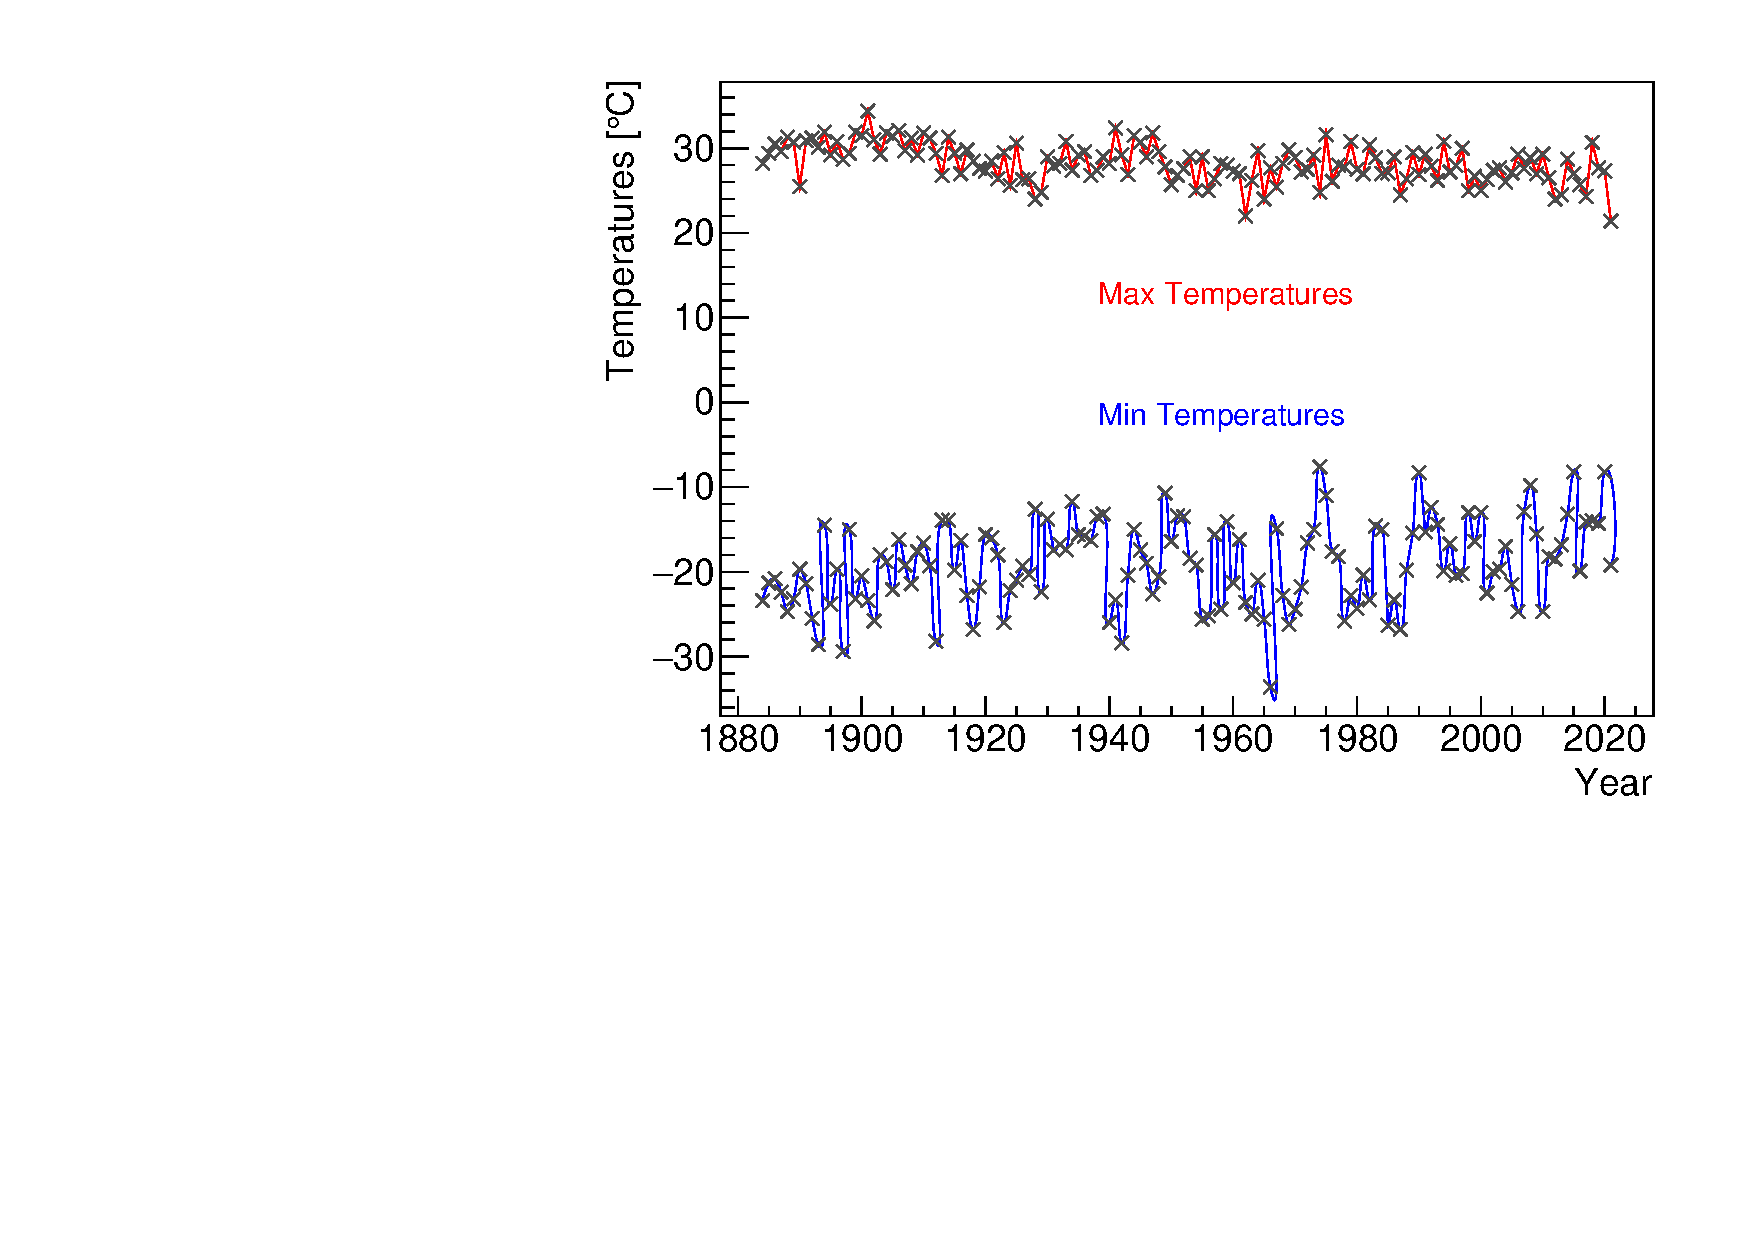
\includegraphics[width=0.5\linewidth]{Images/minmax_Boras.pdf}}
     \subfloat[Umeå]{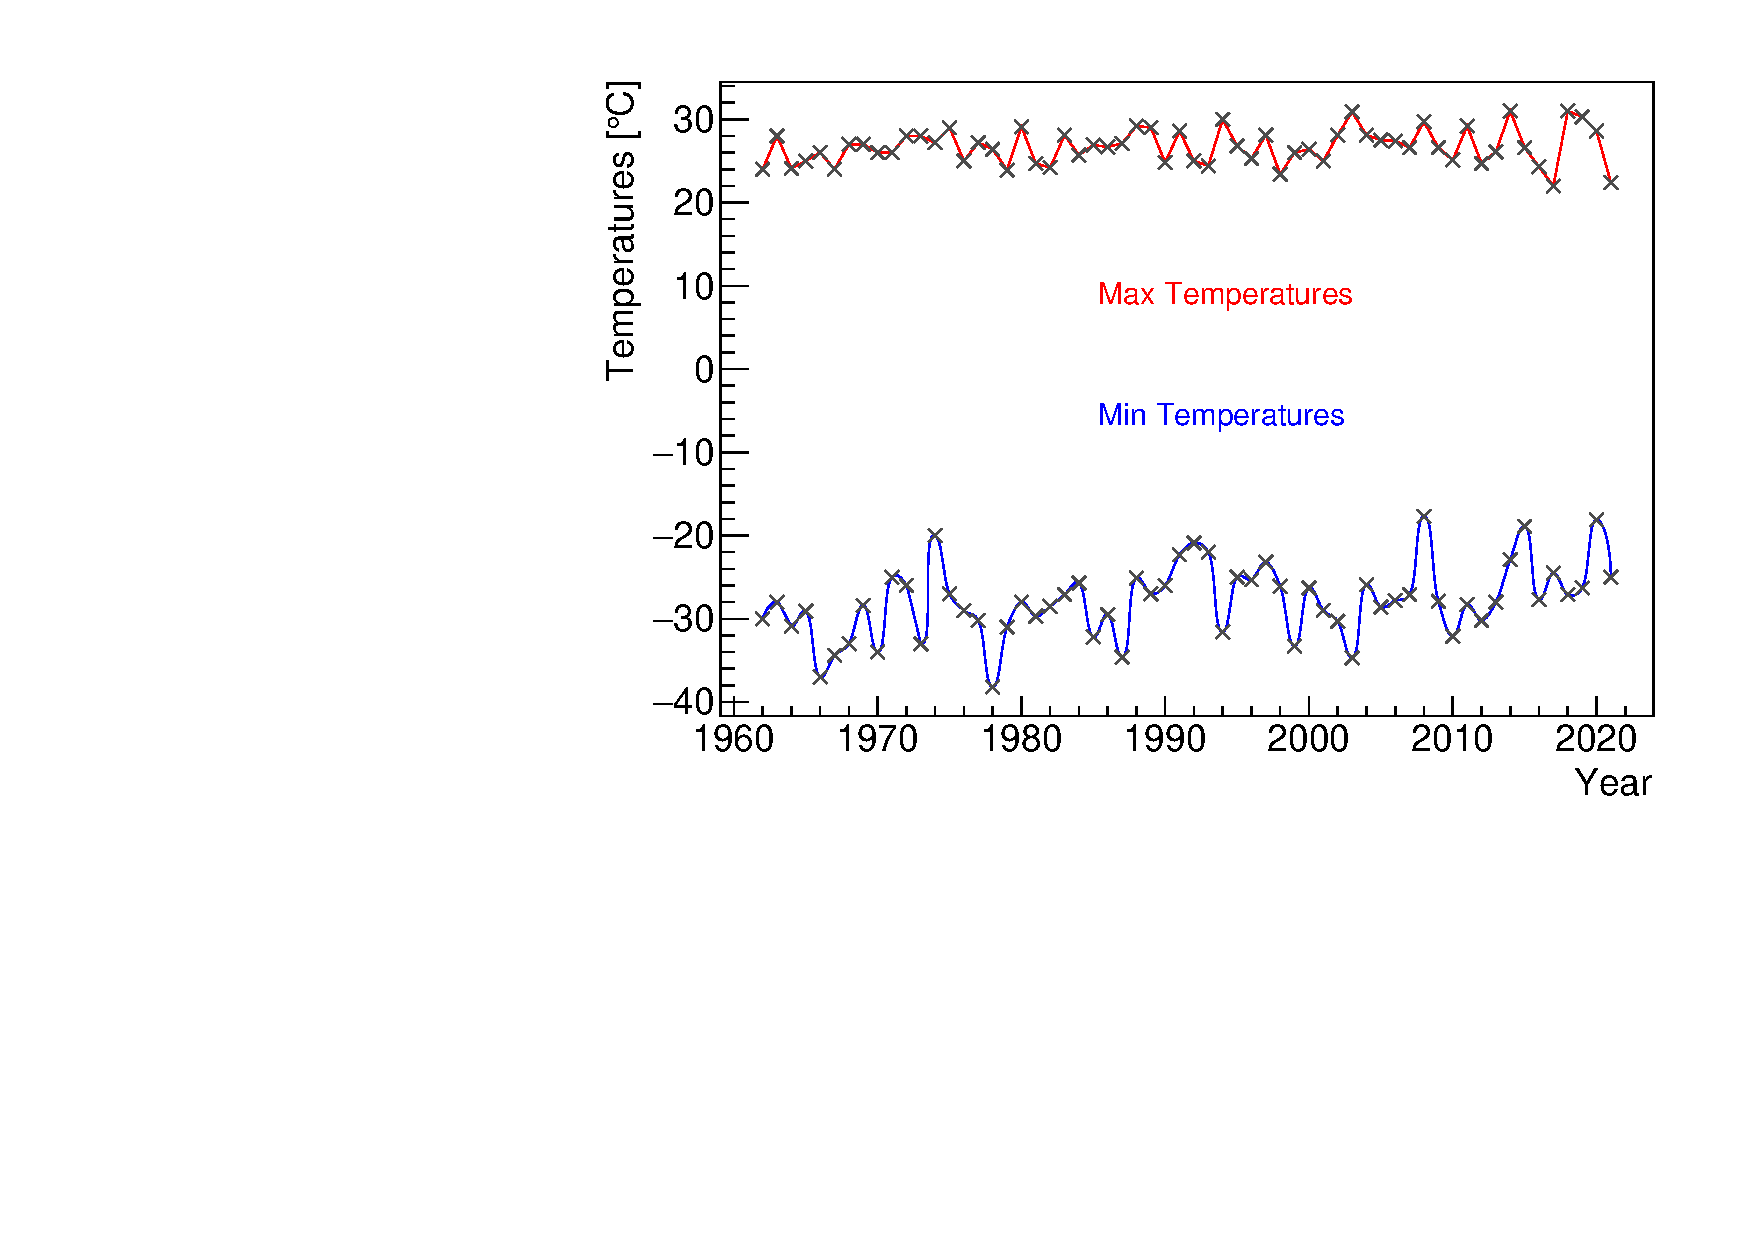
\includegraphics[width=0.5\linewidth]{Images/minmax_Umea.csv.pdf}}
    \caption{Plots illustrating how the maximum and minimum temperatures change throughout time in (a) Falsterbo, (b) Lund, (c) Borås and (d) Umeå.}
    \label{fig:MinMaxTemp}
\end{figure}
As can be seen in the figures above, both the maximum and minimum temperatures fluctuate over time. Furthermore, between adjacent years, the minimum temperature oscillates more. In general, for all the cities, the hottest days reach a temperature of 20-30$^{\circ}$C, whereas the coldest temperature drops as we go more in the North of Sweden; Falsterbo and Lund reach a minimum of -20$^{\circ}$C, while Umeås temperature drops to -40$^{\circ}$C.
\newline
\newline
Also, at the plot for Lund, one can notice a spike in the Max temperature. This is because in that particular year the temperature data recorded were less than usual, which gave us less information.



\subsection{Average daily temperature and season length}
The following figures in this section all correspond to weather data gathered from Lund and Umeå, these two cities are here chosen to showcase the results as they represent different parts of Sweden, where Lund is located in southern Sweden and Umeå is located in northern Sweden. By then plotting the average daily temperature in Lund and Umeå through time, the following plots were obtained.
\begin{figure}[H]
    \centering
    \subfloat[Lund]{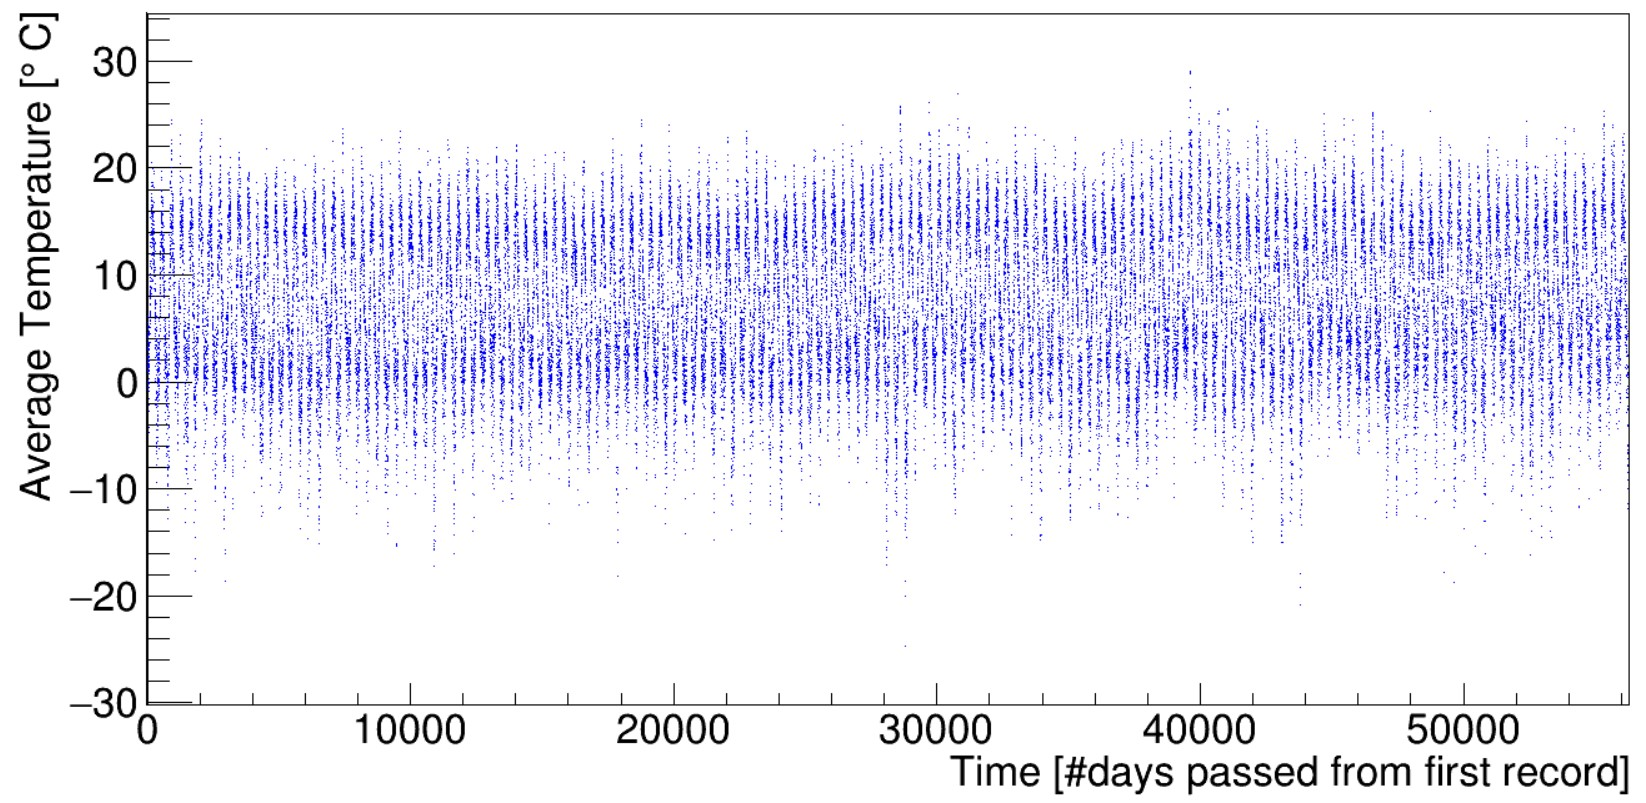
\includegraphics[width=\linewidth]{Images/Lund-daily2.png}}
    \quad
    \subfloat[Umeå]{\includegraphics[width=\linewidth]{Images/Umeå-daily.png}}
    \caption{Plots illustrating how the average daily temperature changes throughout time in (a) Lund, and (b) Umeå.}
    \label{fig:Daily_temp}
\end{figure}
From the plots in Figure~\ref{fig:Daily_temp} it is observed that there seems to be a rather continuous oscillation around a certain temperature for both cities. However, to observe the behavior closer, consider the zoomed-in versions below.
\begin{figure}[H]
    \centering
    \subfloat[Lund]{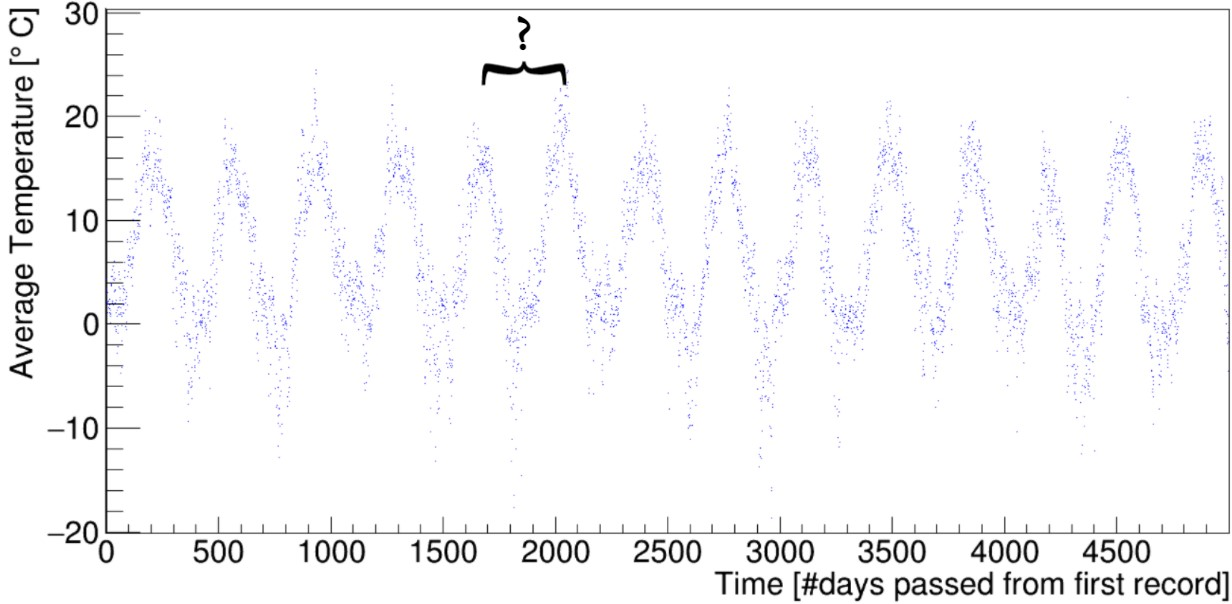
\includegraphics[width=\linewidth]{Images/Lund-daily-zoom.jpg}}
    \quad
    \subfloat[Umeå]{\includegraphics[width=\linewidth]{Images/Umeå-daily-zoom.jpg}}
    \caption{These plots show how the average daily temperature changes throughout the first 5000 days of recorded temperature measurements in (a) Lund, where "?", marks the season length (i.e. time from warmest day of a year to another), and (b) Umeå.}
    \label{fig:Daily_temp_zoomed}
\end{figure}
By considering the results seen in Figure~\ref{fig:Daily_temp_zoomed}, it is apparent that the average daily temperature is changing with a sinusoidal behavior in both of the considered cities. 

To answer the question whether the length of the seasons are changing or not, the distance (i.e. number of days) between each maximum in the plots from Figure~\ref{fig:Daily_temp} are considered. The results are seen below.
\begin{figure}[H]
    \centering
    \subfloat[Lund]{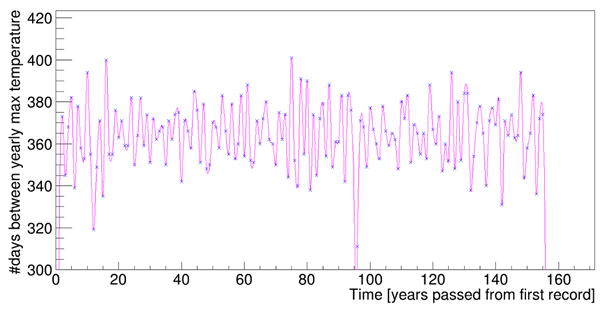
\includegraphics[width=.9\linewidth]{Images/Lund-season-length.png}}
    \quad
    \subfloat[Umeå]{\includegraphics[width=.9\linewidth]{Images/Umeå-season-length.png}}
    \caption{The plots displays how many days that passes between each yearly maximum temperature in (a) Lund, and (b) Umeå.}
    \label{fig:season_length}
\end{figure}

Note that Figures \ref{fig:Daily_temp}-\ref{fig:season_length} all correspond to weather data collected in Lund and Umeå, however, similar behavior as seen in these figures was also observed in all of the investigated data sets.